
\documentclass[11pt]{article}
\usepackage{graphicx}%

\setlength{\oddsidemargin}{0in} \setlength{\evensidemargin}{0in}
\setlength{\textwidth}{6.5in} \setlength{\topmargin}{0in}
\setlength{\headsep}{0in} \setlength{\parskip}{0.1cm}
\pagestyle{plain} \setlength{\textheight}{9.0in}
%end of preamble
\renewcommand{\baselinestretch}{1.0}
\newcommand{\be}{\begin{equation}}
\newcommand{\ee}{\end{equation}}
\newcommand{\bea}{\begin{eqnarray}}
\newcommand{\eea}{\end{eqnarray}}
\newcommand{\nn}{\nonumber}
\newcommand{\bd}{\begin{description}}
\newcommand{\ed}{\end{description}}
\newcommand{\bc}{\begin{center}}
\newcommand{\ec}{\end{center}}
\newcommand{\mysection}[1]{\vspace{.05in} \noindent {\bf  #1}\\ \indent}
\newcommand{\mysubsection}[1]{\vspace{0in} \noindent {\bf #1}\\ \indent}
\newcommand{\mynotationsubsection}[1]{\vspace{.05in} \noindent {\bf #1} \indent}
\newcommand{\myreferencessection}[1]{\vspace{.05in} \noindent {\bf #1} \indent}
\newcommand{\mysubsubsection}[1]{\vspace{.05in} \noindent {\bf #1}\\ \indent}
\renewcommand{\baselinestretch}{2}

\begin{document}
\begin{center} Managing Projects with Uncertain Deadlines
\end{center}
\begin{center}
Robert F. Bordley, Professor and Program Director, University of Michigan Ann Arbor, rbordley@umich.edu \\
Jeffrey M. Keisler, Professor, University of Massachusetts Boston, Boston, MA 02125, jeff.keisler@umb.edu \\
Tom M. Logan, University of Michigan, Ann Arbor, MI 48109, tomlogan@umich.edu
\end{center}
\begin{abstract}
Conventional project management assumes that the required project completion time is known upfront.  But in reality, the required project completion time is often uncertain.  Project management currently addresses this uncertainty with change control processes.  There are other ways of addressing this uncertainty in project management which require significant changes in project management procedures.  Because of the widespread acceptance of project management, introducing such significant changes could be disruptive. This paper presents a much simpler way of incorporating uncertainty in project completion time which requires no changes in conventional project management. \\
\bf Key Words: \rm Decision Analysis, Project management, Project scheduling, Uncertainty modelling
\end{abstract}
\section {Introduction}
         Project management (Kerzner, 2009; Meredith and Mantel, 2003) is a management discipline receiving continuously growing attention and being applied in an increasing number of organizations (Leus, Wullink, Hans and Herroelen, 2003).  Project management creates deliverables for its stakeholders by identifying and managing the various project activities that must be completed in order to create these deliverables.   A large portion of project management practice is based on what we shall term conventional project management heuristics (Klastorin, 2003; Project Management Institute, 2013; Miller, 1963), in particular, the Performance Evaluation and Review Technique (PERT), the Critical Path Method (CPM) and the Graphical Evaluation and Review Technique (GERT). \par
           CPM focuses on specifying the project completion time as a function of the duration of each of the project's activities.  In project scheduling, a path is a sequence of project activities from the start of the project to the completion of the project.  The completion time for a path is a sum of the durations of the activities along that path.   There are typically many paths through the project with the critical path being the path which finishes last.   Because CPM assumes the completion time of each activity is known, the project completion time is simply the completion time of the critical path.  CPM also assumes that the required project completion time (or deadline) and project budget is known to the project manager.  If the project currently finishes after the deadline, the project manager can typically reduce project completion time by `expending extra resources on activities on the critical path' (which is referred to as `crashing').  
         \par PERT and GERT generalize CPM by allowing members of the project team to be uncertain about the time and cost needed to complete the various activities (Kamburowski, 1996; Sculli, 1989; Golenko-Ginzburg, 1989).  If  $U,L,m$ are the pessimistic, optimistic and most likely estimates of an activity's completion time, PERT specifies the uncertainty about the completion time by a beta distribution where the mean completion time of an activity is $\frac{U+4*m+L}{6}$ and the standard deviation of that activity's completion time being $\frac{U-L}{6}$.  There are other ways e.g., decision analytic methods, for specifying an activity's completion time (Keefer and Verdini, 1993), or other more flexible alternatives to the beta distribution (Perez, Martin, Garcia and Granero, 2016).
         Since the duration of each activity is uncertain, the completion time of each path --- which is the sum of the completion time of the activities along that path --- is uncertain.  As a result, project management focuses on the probability of the project, and thus the probability of all the paths in that project, finishing before its deadline.  PERT defines the critical path as the path with the greatest mean completion time and assumes that the project, and all its paths, finish when the critical path finishes.  Because PERT also assumes the critical path completion time is normally distributed and that all activity durations are independent, PERT is able to specify the probability of the project finishing on time as a simple function of the difference between the deadline and mean critical path completion time divided by the standard deviation of that difference.
         \par
         GERT allows for more general distributional assumptions and project networks than PERT.  However GERT, while generalizing CPM to allow for uncertain project completion times, still presumes that the project's stakeholders have specified definite (i.e., certain) requirements for the overall project's completion time at the start of the project.  But it is well known that these and other requirements change because of unforeseen changes in stakeholder needs (Ward and Chapman, 2003; Huemann, Turner and Keegan, 2007; Bordley and Keisler, 2015). As a result, project management provides a change control process which allows stakeholders to modify deadlines and other requirements after the start of the project.  This process is reactive in requiring the project manager to treat requirements as fixed --- until such time as a change control process adjusts the deadline and leads to a change in project plan (Calhoun, Deckro, Moore, Chris and Hove, 2002). But while this change control process reduces some of the disruption caused by specification changes,  change is still disruptive and typically requires that some previous work be redone or discarded.  To reduce the amount of rework, agile approaches (Maylor,  Vidgen and Carver, 2008) attempt to restructure the work flow so that the project manager knows how particular specifications will change before undertaking extensive work.  This approach attempts to address requirement uncertainty by eliminating or mitigating that uncertainty.  While this approach recognizes that stakeholder understandings of their own requirements may deepen as the deliverable is developed, it generally requires more frequent iterations with the stakeholders. Related approaches recognize that uncertain performance in some activities affects the needed performance across other activities, and techniques such as active monitoring and corrective action (Hu,Cui, Demeulemeester and Bie, 2016), or generation of options (Creemers, De Reyck and Leus, 2015) are used to speed the response to such changes. However agile approaches frequently require costly and time-consuming changes in conventional project management (Schwaber, 2004).  They also assume that stakeholder uncertainty about their requirements will substantially diminish over time as the deliverable is developed.
          \par
          But the conventional and agile approaches to project management still require the project team to treat requirements as fixed until they are officially changed.   This paper proposes making the project team's decision making more robust by enabling them to incorporate their uncertainty about their requirements in their project decision making.   There are, of course, a wide variety of decision tools that can already be used to make uncertain decisions  (Ding and Zhu, 2015; Elmaghraby, 2003; Morgan and Henrion, 1992;  Chapman and Ward, 1997; Clemen, 1996; Khodakarami, Fenton and Neil, 2007; Pich, Loch and DeMeyer, 2002).    
Many of these common decision analysis methods are already recognized in the PMBOK.  And, in fact, these methods are often use by the project manager in addressing uncertainty associated with the duration, cost and feasibility of various activities in the project.  To build on these techniques for managing uncertain activities, this paper will simply introduce an artificial activity into the project which reflects requirement uncertainty.  This seamless integration of requirements uncertainty management into conventional project management will lead to project decisions more robust to requirement uncertainty.
\par
This approach does not aim to reduce the uncertainty in those requirements (which is the aim of change control and agile processes.).  As a result, the value which the propose solution adds to project management is the expected value of including uncertainty and not the expected value of imperfect information.  But Morgan and Henrion (1982) demonstrate how the expected value of including uncertainty can often be significant.
          This third approach focuses on impacting the wide variety of decisions (e.g. crashing decisions) which the project team makes in the course of the project.   In making these decisions, the project team already recognizes the uncertainty in activity duration times and what is technically feasible while assuming requirements are fixed.  Consistent with decision analysis, our approach argues that the project team should also recognize the very real uncertainty about whether existing requirements will change.   A manager who recognizes requirement uncertainty will typically make different decisions then a manager who assumes requirements are fixed.  \par
            This paper focuses on a particular kind of requirement uncertainty, deadline uncertainty, whose important is highlighted by the substantial research on make-span minimization (Kolish and Padman,2000). This approach builds on the established project management tradition of introducing fictitious or dummy activities with zero expected duration to the activity network (e.g., Neumann and Zimmerman, 1999; Estevez-Fernandez, 2012). However this paper's use of dummy activities will be different from the traditional use of dummy activities.  The first two sections of the paper present our approach.  Later sections then show how use of this approach can often substantially improves the probability of project success.   \par
           While this approach is applicable to both PERT and GERT and Agile project management, this paper will focus on its application to a project managed using PERT.  By addressing deadline uncertainty in PERT, this paper will eliminates one of PERT's most widely noted limitation.   But because our approach is directly applicable to any project management system which treats deadlines as fixed, it can also be extended to risk-based project management approaches other than PERT (Zafra-Cabeza, Ridao and Camacho, 2008; Herroelen and Leus, 2003; Herroelen and Leus, 2005) which do not assume normally distributed path completion times.   
           \par
The next section presents the solution.  The third section discusses how this solution can improve the quality of certain management decisions.  The fourth section constructs a model quantifying the benefits of this approach.  The fifth section discusses the limitations of PERT methods compared to more modeling intensive methods, and whether these limitations affect the benefits of our approach.  To demonstrate the advantages of this approach, the sixth  randomly generated projects using Monte Carlo simulation.
\section{Proposed Solution}
\subsection{Motivation}
First consider the following motivating example. Suppose the stakeholder, upon receiving the deliverables from the manager's project, immediately starts a 'complementary' activity designed to use those deliverables to finish some longer term project.  When the manager's project and this complementary activity are finished, the longer-term project is finished.   Suppose the longer-term project has a fixed required completion time $r_O$.   If the completion time of the complementary activity were known to be $t$, then the stakeholder could give the manager's project a fixed deadline of $r=r_O-t$ which would then allow the stakeholder to meet their deadline of $r_O$. \par
But suppose the completion time of the complementary activity is uncertain. Then the required completion time, $r$, for the manager’s project will be uncertain.   So the stakeholder cannot give the manager a fixed deadline for the original project.\par
\begin{figure}[h]
\begin{center}
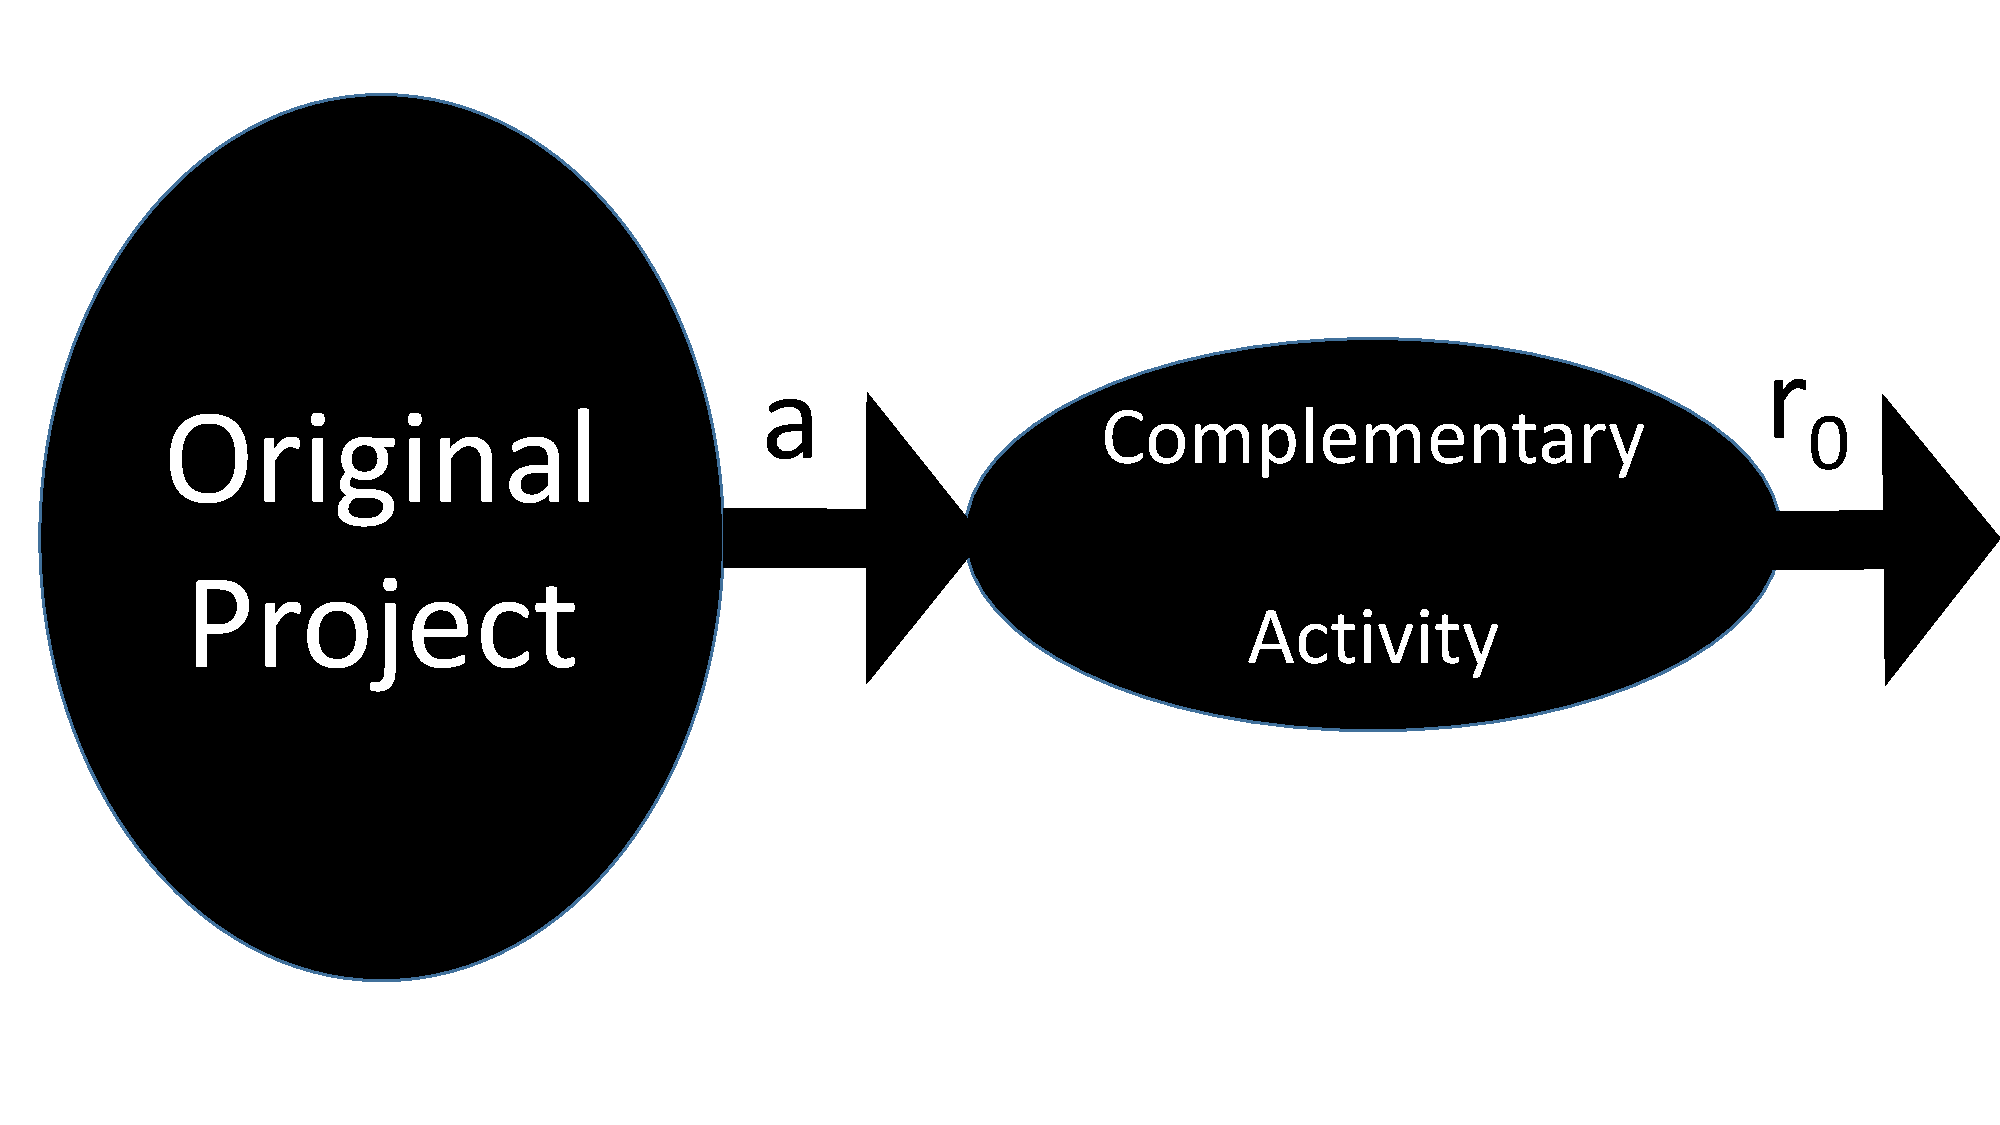
\includegraphics[scale=0.30]{uncertaindeadlines.pdf}
\caption{The Original Project embedded in the Manager's Project}
\label{fixXscaled}
\end{center}
\end{figure}
          Fortunately, the manager could simply re-define the actual project so that it finishes when the longer term project finishes.    This enlarged project will have the same required completion time $r_O$ as the stakeholder's long-term project.   The project network describing the new project consists of the network for the original project plus an additional activity, corresponding to the complementary activity, which can only start after all the activities in the original project have finished.  But while the manager may be able to affect the completion time of the activities in the original project by adding resources, the manager will not be able to affect the completion time of this complementary activity. \par
          If the completion time of the complementary activity is $t$ and if the actual completion time of the manager's project is $a$, then the completion time for the redefined project will be $a+t$.   The project will finish on time when $a+t \leq r_O$.    Because $t$ is uncertain, the project manager needs the stakeholder to specify an optimistic completion time, $t_O$, for the complementary project, as well as a pessimistic completion time $t_P$  and a most likely completion time, $t_L$.  Once $t_O$, $t_L$ and $t_P$ are specified, the manager can then use standard PERT-CPM methods to model the probability of the redefined project finishing by its new deadline $r_O$ (which is just the probability that $a+t \leq r_O$.)   The uncertainty in the deadline of the original project is completely determined by the uncertainty in the complementary activity.   (The uncertainty in the actual completion time, $a$, of the original project is, of course, described by the uncertainty in the activities within the original project.)  Since the manager is now responsible for a redefined project including the complementary activity, the manager will make decisions that appropriately recognize the uncertainty in the required completion time for the original project.
\subsection{Extension to General Projects}
          We now show how the solution for the special case just described can be extended to the more general case where there is no longer-term project but the stakeholder is still uncertain about the time when the project must finish.  Let $r_O$, $r_L$ and $r_P$ be the stakeholder's estimate of the latest possible project deadline, the most likely project deadline and the earliest project deadline.  Define $t=r_O-r$ where $r$ is the uncertain required completion time for the project.  Then $t$ will have a maximum possible (pessimistic) value of  $t_P = r_O-r_P$ , a most likely value of  $t_L = r_O-r_L$ and a minimum (optimistic) value of   $t_O = r_O-r_O=0$.  The manager's project will finish on time if $a < r $ (which implies $a+t < r_O$. )  Hence, making decisions to maximize the probability of $a+t$ being less than $r_O$ will be equivalent to making decisions to maximize the probability of the original project having a completion time, $a$, which is earlier than its original uncertain deadline, $r$.  \par
          To model this with the classical project management structure, i.e., an activity network, the manager re-defines the original project to have a deadline $r_O$ and to include a fictitious complementary activity with uncertain completion time $t$ which starts when all other activities finish.   Fictitious activities have been used, for other purposes, in other project management contexts (Vanhoucke (2013), pg. 244; Schwindt (2005), pg.8).  The classical project management solution to the original project supplemented with this added activity will be the appropriate solution to the original project where the stakeholder's completion time was uncertain.
\section{Why Ignoring Deadline Uncertainty Misleads Project Managers}
First consider the simplest case (CPM) with no uncertainty about the duration of each activity and the project manager ignoring deadline uncertainty by treating the deadline as if it equalled the median deadline.   Then if the manager scheduled activities to finish exactly at this estimated deadline, the project manager would conclude the probability of on-time completion was $100\%$ even though it was actually only $50\%$.  So ignoring deadline uncertainty can dramatically overestimate the on-time completion probability.\par
To consider the general case where there is uncertainty about project completion time,  let $X_i$ represent the uncertain completion time of path $i$ with $T$ representing the uncertain deadline.  This paper will use the term slack to describe $T-X_i$ which is the uncertain amount by which path $i$ finishes ahead of the deadline.  Let $e_i$ and $v_i$ be the mean and variance of this uncertain slack.  The probability of path $i$'s on-time completion is
$$ p_i= P(X_i \leq T) = P(T-X_i \geq 0) = P(\frac{T-X_i-e_i}{\sqrt{v_i}} \geq - \frac{e_i}{\sqrt{v_i}}) =
P(\frac{e_i-(T-X_i)}{\sqrt{v_i}} \leq \frac{e_i}{\sqrt{v_i}})  $$
Let $\eta_i=\frac{e_i-(T-X_i)}{\sqrt{v_i}}$ and $z_i=\frac{e_i}{\sqrt{v_i}}$ and let
$F_i$ be the cumulative distribution of $\eta_i$.  Then $p_i=P(\eta_i \leq z_i)=F_i(z_i)$. \par   
Suppose the manager who ignores the variance in the deadline estimates the deadline $t$ as the mean of $T_i$.  Then the mean value of $t-X_i$ is $e_i$ and the variance is $v^*_i<v_i$.    The manager will estimate the probability of on-time project completion as 
$$ p^*= P(\frac{e_i-(t-X_i)}{\sqrt{v_i}} \leq \frac{e_i}{\sqrt{v^*_i}})  $$
Let $\eta^*_i=\frac{e_i-(t-X_i)}{\sqrt{v^*_i}}$ and suppose that $\eta^*_i$ also has cumulative distribution $F_i$.   Then if $z^*_i= \frac{e_i}{\sqrt{v^*_i}})$, $p^*_i=F_i(z^*_i)$.  Then
\begin{itemize}
\item if $e_i>0$, then $z_i$ and $z^*_i$ are positive and $p_i=F(z_i) \leq F(z^*_i)=p^*_i$. Ignoring deadline uncertainty will lead to overestimation of path $i$'s probability of on-time completion.
\item if $e_i<0$, then $z_i$ and $z^*_i$ are negative and $p_i=F(z_i) \geq F(z^*_i)=p^*_i$. Ignoring deadline uncertainty will lead to underestimation of path $i$'s probability of on-time completion.
\end{itemize}
To adjust the probability of the project finishing on-time, the manager can reorganize specific activities by adding (or subtracting) resources from them.  When the manager adds resources, this is commonly referred to as the `crashing' decision.  Suppose the manager wishes to add just enough resources to increase path $i$'s on-time completion probability to equal some threshold $\alpha$.  Ignoring ignoring deadline uncertainty (when $e_i>0$) will lead the manager to add an insufficient level of resources and fall short of that goal.\par
But ignoring deadline uncertainty also distorts decisions about which path to crash.  Suppose the manager must choose between crashing path $i$ or path $j$ and always chooses to crash the path with the greatest schedule risk. For simplicity, suppose for this case only, that $F_i=F_j$.  
 Then the manager should crash path $i$ over $j$ if $$F_i(\frac{e_i}{\sqrt{v_i}}) \leq F_i(\frac{e_j}{\sqrt{v_j}}) \Longrightarrow \frac{e_i}{e_j} \leq \sqrt{\frac{v_i}{v_j}}$$
But the manager who ignores deadline uncertainty will crash $j$ over $i$ if  $\frac{e_i}{e_j} \geq \sqrt{\frac{v^*_i}{v^*_j}}$.
Thus the manager who ignores deadline uncertainty will make decisions contrary to the manager who recognizes requirement uncertainty when 
$$\sqrt{ \frac{v_i}{v_j}} \geq \frac{e_i}{e_j} \geq \sqrt{\frac{v^*_i}{v^*_j}}$$
If $v$ is the variance of deadline uncertainty, then this condition implies
$$ \frac{v^*_i+v}{v^*_j+v} \geq \frac{e^2_i}{e^2_j} \geq \frac{v^*_i}{v^*_j}   
\Longrightarrow   (1+\frac{v}{v^*_i})  \geq 1 + \frac{v}{v^*_j}  
\Longrightarrow  v^*_i \leq v^*_j $$
This shows that the manager who ignores deadline uncertainty will have a bias toward crashing paths with higher completion time variance. Hence ignoring deadline uncertainty overestimates project completion time and leads to inappropriate resource allocation decisions.
\section{Quantifying the Benefits of Recognizing Deadline Uncertainty}  
\subsection{Modeling Project Completion Time}
 To quantify the impact of these biases, number the paths in the project $i=1,...k$. 
 The probability of the project finishing on time is the probability that $T-X_i \geq 0, i=1,...,k$ which is the same as the probability
 $\eta_1,...\eta_k \leq z_1,...z_k$ . Let
 $F$ be the multivariate cumulative distribution of $\eta_1,....\eta_k$ so that the probability of on-time completion is
 $p=F(z_1,...,z_k)$. For the manager who ignores deadline uncertainty, the probability is
$p^*=F(z^*_1,....z^*_k)$. \par
Each path in the project is made of several activities, some of which may be shared by other paths.
Number the activities in the project $m=1,....M$ and let $\pi_m$ be the amount of resources associated with crashing activity $m$.   In some cases, crashing of an activity significantly reduces its completion time.  In other cases, it introduces confusion into the project and may significantly increase its completion times.  To model this, we assume \\
\bf Assumption 1: \rm Crashing activities $1...m$ while it reduces their mean duration will introduce uncertainties, uncorrelated with any other project uncertainties, which increase the variance of the activity's duration.  \\
Specifically suppose that optimally spending $\pi_1,...\pi_M$ on crashing activities $1,...m$ respectively reduces the mean duration by $x_1,....x_M$ respectively and increases the variance of duration by $\sigma^2_1,...\sigma^2_M$ respectively.
Let $I_{jm}=1$ if activity $m$ is on path $j$ with $I_{jm}=0$ otherwise. If $e^0_j$ and $v^0_j$ are the mean and variance of $T-X_j$ prior to crashing, then spending resources $\pi_1,...\pi_M$ on crashing leads to the following revised values of $e_j$ and $v_j$:
\begin{eqnarray*}
e_j &=& e^0_j+\sum_m x_m I_{jm}, j=1...k \\
v_j &=& v^0_j+\sum_m I_m \sigma^2_m, j=1...k
\end{eqnarray*}
Since $\sigma^2_m$ and $x_m$ are both increasing functions of only $\pi_m$, it is convenient to rewrite $\sigma^2_m$ as only a function of $x_m$.   As a result, the problem of choosing $\pi_1,...\pi_M$ to maximize the on-time completion probability can be rewritten as the problem of choosing $x_1,....x_M$ to maximize $\ln(p)$.\par 
 The first-order Kuhn-Tucker conditions for $x_1,...x_M$ are
$$\frac{\partial \log p}{\partial x_m} = \sum_{j=1}^k \frac{\partial \log F(z_1,...z_k)}{\partial z_j} 
\frac{\partial z_j}{\partial x_m} =0  , m=1,...M $$
where
$$ \frac{\partial z_j}{\partial x_m} = \frac{1}{\sqrt{v_j}} \frac{\partial e_j}{\partial x_m}-  
\frac{1}{2} e_j v_j^{3/2} \frac{\partial v_j}{\partial x_m}]  \mbox{ and } \frac{\partial e_j}{\partial x_m}=1  $$
Note that all $M$ equations are satisfied if it is possible to choose $x_m$ so that
\begin{equation} 
\frac{\partial z_j}{\partial x_m} = (1/\sqrt{v_j}) [1 -   \frac{e_j}{2 v_j}  \frac{\partial v_j}{\partial x_m}] =
\frac{v_j^{-3/2}}{2}[2v_j - e_j \frac{\partial v_j}{\partial x_m}  ] 
 \label{firstorder}
\end{equation}
\subsection{Second-order Optimality Conditions}
The first-order condition will only define an optimal solution if the second-order condition is satisfied.
Three assumptions will be made to ensure the second-order condition is satisfied.  The first assumption is: \\
\bf Assumption 2: \rm The coefficient of variation of the uncertainty induced by crashing activity $m$ is some constant $s_m$ independent of $x_m$ which may vary from activity to activity \\ 
Then 
$\frac{\sigma_m}{x_m}=s_m$, $\sigma^2_m=x^2_m s^2$ and $\frac{\partial v_j}{\partial x_m} = 2 x_m s^2$.  Substituting into the first-order conditions gives
\begin{eqnarray*}
\frac{\partial z_j}{\partial x_m} &=& \frac{v_j^{-3/2}}{2}[2v_j - e_j \frac{\partial v_j}{\partial x_m}] \\ &=&
\frac{v_j^{-3/2}}{2}[2v^0_j + 2 \sum_m I_{mj} x^2_m s^2 -  (e^0_j + \sum_m I_{mj} x_m) 2 x_m s^2_m)]  \\
&=& v{j^{-3/2}} [v^0_j-x_m s^2_m e^0_j] 
\end{eqnarray*}
which is satisfied if 
$$ x_m =   \frac{ v^0_j}{s^2_m e^0_j}  $$
So the mean reduction in activity $m$ when the mean completion time is large (and $e^0_j$ is smaller), when the variance of the activity is large and when the uncertainty induced by crashing is smaller.   \par
The second assumption made to ensure concavity is:
\\ \bf Assumption 3: \rm  $\ln(p)$ is concave in $z_1,...z_k$. \\
 This assumption will be true for log-concave densities like the normal distribution, extreme value distribution, the Laplace distribution, the logistics distribution, the uniform and exponential distribution as well as for many other distributions whose density is not log-concave (or are only log-concave for certain parameter settings.) \par
Assuming $\ln(p)$ is concave in $z_1,...z_k$ does not imply it is concave in $x_1,...x_k$. \par  To ensure that $ln(p)$ is concave in $x_1,...x_k$, this paper will additionally require that the Hessian matrix $\frac{\partial^2 z_j}{\partial x_m \partial x_{m*}} \geq 0$, be negative definite.   To determine the circumstances under which this condition is satisfied, define 
$A_j=[v^0_j - x_m s^2_m e^0_j] $ so that $\frac{\partial z_j}{\partial x_m} = v_j^{-3/2} A_j $.  Then
$$\frac{\partial^2 z_j}{\partial x_m \partial x_{m*}} =  \frac{\partial v_j^{-3/2}}{\partial x_{m*}} A_j +
 v_j^{-3/2} \frac{\partial A_j}{\partial x_{m*}}  $$
Evaluating this derivative at the point where the first-order condition is satisfied gives
$$
\frac{\partial^2 z_j}{\partial x_m \partial x_{m*}} = v_j^{-3/2}\frac{\partial A_j}{\partial x_{m*}} 
=  - s^2_m e^0_j \mbox{ for } m=m^* \mbox{ and } = 0  \mbox{ for } m \neq m^* $$
      If $e^0_j \geq 0$,  then the diagonal elements of the matrix, $\frac{\partial^2 z_j}{\partial x^2_m} $ is negative while the off-diagonal elements equal zero.  Hence the matrix is negative definite and the second-order condition is satisfied if we this third assumption: \\
      \bf Assumption 4: \rm  Prior to crashing, the mean duration of each path is less than the mean deadline ($e^0_j \geq 0$).   \\
If this condition were not true, then the project prior to crashing would --- in the absence of uncertainty in both deadlines and activity durations --- always run late.  In our view, it is not unreasonable to rule out such a possibility.    
\par
Since the concavity conditions are satisfied, the solution of the first-order conditions,
\ref{firstorder}, $x_m=\frac{v^0_j}{s^2_m e^0_j}$ is an optimum.
\subsection{Computation of Schedule Risk}
The first-order conditions imply $$e_j=e^0_j+\sum_m I_{mj} x_m = e^0_j +\frac{v^0_j}{e^0_j} \sum_m \frac{I_{mj}}{s^2_m} $$
Define $a_j=\sum_m \frac{I_m}{s^2_m}$ so that $$e_j=e^0_j + \frac{v^0_j}{e^0_j} a_j$$. In addition
$$ v^0_j + \sum_m I_{mj} (x_m s_m)^2 = v^0_j + \sum_m I_{mj} (\frac{v^0_j}{s^2_m e^0_j} s_m)^2 =
v^0_j + (\frac{v^0_j}{e^0_j})^2 \sum_m \frac{I_{mj}}{s^2_m} $$ so that
$$v_j= v^0_j + (\frac{v^0_j}{e^0_j})^2 a_j $$ 
Then
\begin{eqnarray*}
z_j &=& \frac{e^0_j + \frac{v^0_j}{e^0_j} a_j}{\sqrt{v^0_j+(\frac{v^0_j}{e^0_j})^2 a_j }} 
= \frac{\frac{e^0_j}{\sqrt{v^0_j}} + \frac{(v^0_j)^{1/2}}{e^0_j} a_j}{\sqrt{1+ \frac{v^0_j}{(e^0_j)^2} a_j }} 
= \frac{ z^0_j + \frac{a_j}{z^0_j}}{\sqrt{1+ \frac{a_j}{(z^0_j)^2}}}  \\
&=& z^0_j \frac{1 + \frac{a_j}{(z^0_j)^2}}{\sqrt{1+ \frac{a_j}{(z^0_j)^2}}} 
= z^0_j \sqrt{1 + \frac{a_j}{(z^0_j)^2}}   
=   \sqrt{(z^0_j)^2 + a_j}
\end{eqnarray*}
with the on-time completion probability for a manager who recognizes deadline uncertainty being  
$p=F(z_1,...z_k)$ using, for example, the technique described in the first two sections of this paper.  \par  
Now consider the manager who ignores deadline uncertainty
 Let $\kappa=
\frac{v^*_j}{v^*_j+v}$ so that $1-\kappa$ represents the fraction of the variance in $T-X_j$ neglected by the manager who ignores deadline uncertainty.   This manager sets the mean reduction in activity $m$' duration to be
$$x^*_m=\frac{v^*_j}{s^2_m e^0_j}=\frac{v^*_j}{v^0_j} \frac{v^0_j}{s^2_m e^0_j} =  \kappa x_m < x_m$$
As a result, 
\begin{eqnarray*}
e^*_j &=& e^0_j+\kappa \sum_m I_{mj} x_m = e^0_j + \kappa a_j \frac{v^0_j}{e^0_j} < e_j \\
 v^*_j &=& v^0_j + \sum_m I_{mj} (\kappa x_m s_m)^2 = v^0_j + \kappa^2 a_j (\frac{v^0_j}{e^0_j})^2 < v_j 
 \end{eqnarray*}
 Then
\begin{eqnarray*}
z^*_j &=& \frac{e^0_j + \kappa \frac{v^0_j}{e^0_j} a_j}{\sqrt{v^0_j+\kappa^2(\frac{v^0_j}{e^0_j})^2 a_j }]} 
= \frac{ z^0_j + \kappa \frac{a_j}{z^0_j}}{\sqrt{1+ \kappa^2 \frac{a_j}{(z^0_j)^2}]}}   \\
&=& z^0_j \frac{1 + \kappa \frac{a_j}{(z^0_j)^2}}{\sqrt{1+ \kappa^2 \frac{a_j}{(z^0_j)^2}]}} 
=  \frac{(z^0_j)^2 + \kappa a_j}{\sqrt{(z^0_j)^2+ \kappa^2 a_j }}  
\end{eqnarray*}
 Note that $z_j \geq z^*_j$ when 
 $$\sqrt{(z^0_j)^2+a_j} \geq \frac{(z^0_j)^2 + \kappa a_j}
 {\sqrt{(z^0_j)^2+\kappa^2 a_j}}  \Longrightarrow ((z^0_j)^2+ a_j) ((z^0_j)^2 + \kappa^2 a_j) \geq ((z^0_j)^2 +\kappa a_j)^2  \geq 0 $$
This is true if and only if 
\begin{eqnarray*}
(z^0_j)^4 &+& (z^0_j)^2 (a_j + \kappa^2 a_j) + \kappa^2 a^2_j - [(z^0_j)^4 + 2 (z^0_j)^2 \kappa a_j + \kappa^2 a^2_j] \\ &=& 
  (z^0_j)^2 a_j[(1 + \kappa^2 ) - 2 \kappa] 
  =  (z^0_j)^2 a_j(1-\kappa)^2 \geq 0 
  \end{eqnarray*}
which is always true.  Hence $z_j \geq z^*_j$ and $p=F(z_1,...z_k) \leq p^*=F(z^*_1,...z^*_k) $.  Ignoring deadline uncertainty reduces the project's on-time completion probability. \par
Since both $\kappa$ and $z^0_j$ depend on $v$,   it is useful to define $$z^1_j=\frac{x_j}{\sqrt{v^*_j}}=
\frac{x_j}{\sqrt{v_j \kappa_j}} = \frac{z^0_j}{\sqrt{\kappa_j}} $$ 
which is independent of $v$.   Then 
\begin{eqnarray*}
z_j &=& \sqrt{\kappa_j(z^1_j)^2 + a_j} \\
z^*_j &=&  \frac{ \kappa[(z^1_j)^2+ a_j]}{sqrt{ \kappa[(z^1_j)^2 + \kappa a_j]}} \\  
&=& \sqrt{\kappa} \frac{(z^1_j)^2+ a_j}{\sqrt{(z^1_j)^2 + \kappa a_j}}  
\end{eqnarray*}
so that $z_j,z^*_j$ are functions of $\kappa$ (which measures relative deadline variance), $a_j$ (which measures the ease of crashing path $j$) and $z^1_j$ (which measures all other path attributes.\par
The improvement in on-time completion probability resulting from recognizing deadline uncertainty is $p-p^*$.  When deadline variance is small and $\kappa \approx 1$, $z_j \approx z^*_j, j=1...k$.  When deadline variance is large and $\kappa \approx 0$, $z^*_j \approx 0$ and $z_j=\sqrt{a_j}, j=1...k$.      
\section{Generality of this Approach}
This approach was designed to supplement those project management techniques which presume that the project deadline is fixed.  Our innovation is in showing how uncertain deadlines could be easily integrated into such methods using a dummy activity.  Because PERT is the most well-known example of such a method,  this paper focused on PERT.  But PERT makes many other assumptions which have been criticized.  As this section notes, the benefits of our approach are not contingent on these PERT assumptions being satisfied. \par
Consider first the limitations in PERT's objective function.  PERT focuses on maximizing the probability of finishing the project by the deadline.  But there are many other objectives e.g., the minimization of expected project completion time, the minimization of a weighted average of mean completion time and the variance of completion time, value at risk, etc.   However the results of this paper can be used to enable PERT to maximize the expected utility of completion time for any well-defined Von Neumann-Morgenstern utility.  Specifically, any 
von Neumann-Morgenstern utility can always be interpreted as the cumulative distribution of some possibly latent random variable.  As a result, maximizing  expected utility is equivalent to maximizing the probability of completion time exceeding this latent random variable. If this latent random variable is interpreted as an uncertain deadline, then the methodology in this paper addresses any PERT problem where the objective function is defined by a utility function.\par
Next consider PERT's assumption that the critical path completion time is normally distributed.  While this assumption has some plausibility when the number of activities is large and the correlation between paths is small, there are many realistic examples for which this assumption is inappropriate.  The proposed method of adding a complementary dummy activity does not place any limitation on the distribution used to model path completion times.  And, in fact, the analytic demonstration of the benefits of this approach first focused on the broader family of two parameter distributions before focusing on the normal distribution to develop analytically tractable estimates of the benefits of the method.  But while normality assumptions may be useful in calculating the benefits of this approach, they are not required to achieve the benefits of this approach.\par
 While PERT recognizes that some activities may need to be finished before other `precursor' activities can start, it is not structured to address activities with cyclic dependencies (where one activity requires inputs from a second activity and the second activity provides inputs to the first activity).  Fortunately the design structure matrix methods (Eppinger and Browning, 2012) do address this limitation by showing how cyclic dependencies can be eliminated with typically minimally  adverse impact on the project.  Our approach makes no contribution to this particular problem and assumes that techniques like the design structure matrix have already been used to eliminate cyclic dependencies. \par
PERT assumes each activity will start as soon as all precursor activities are finished.  But if the start of this new activity will monopolize equipment needed by an activity that starts later, starting each activity as soon as possible may delay the project's completion time.  Since this paper shows how our approach can improve resource-allocation decisions (like crashing), the proposed method is potentially useful in these more complex decisions.  \par
Finally PERT assumes project completion time is determined by the completion time of the critical path.  Since the proposed approach creates a complementary activity which starts after every activity is finished, the value of the proposed approach is unaffected by which path actually finishes last. Note also that the family of distributions included in our analysis of the benefits of this approach includes the Gumbel which does describe the asymptotic distribution of the maximum of many path completion times. In fact, if $X$ and $T$ both have Gumbel distributions, their difference is a logistic distribution which is also among the family of distributions considered in our analysis.
Hence our approach is valid even when PERT's critical and distributional assumptions are violated.  \par
But while the validity of our methodology is unaffected by the common limitations associated with PERT, its simplicity makes it especially useful for commonly used network-based methods like PERT.   But there are alternative more complex methods for allocating time and resources to activities.
Stochastic programming based optimization is generally a preferred method for identifying strategies acceptably close to optimal in an acceptable computation time. For example, Resource Constrained Project Scheduling Problems (RCPSP, e.g., Brucker et al, 1999) is a relatively sophisticated method which typically minimizes the expected time to completion (although the literature discusses other possible objectives, e.g. value-at-risk.) Once a problem is thus formulated, it would require little additional effort to instead maximize the probability of meeting a given deadline (or similarly value-at-risk minimization), and even to add an additional dummy uncertain variable for the deadline.   Hence the incremental contribution of the proposed approach to these methods is much smaller than its contribution to methods like PERT or GERT.  \par
But because these methods are harder for most project managers to use,  there is a significant cost to using these methods versus PERT or GERT.  Hence evaluating our approach versus these more complex approaches involves a cost/benefit analysis of how well our enhancement of PERT performs compared to more difficult, but higher performing, stochastic optimization methods.  The next section focuses on this question. 
\section{Simulation Comparison of Alternate Approaches}
There is a trade-off between the ease of implementation and benefit of modified-PERT compared to that for more modelling intensive approaches. Of course, if the project conforms exactly to the assumptions of modified-PERT, additional modelling efforts will not produce any benefit. To explore the usefulness of the proposed approach extends to other situations, we consider a slightly more complicated activity network and simulate in Microsoft Excel the performance of the PERT heuristic against an optimization approach under different assumptions about uncertainty.  \par
Specifically, we consider the activity network shown in Figure $4$, which is a tree with one level of branches of varying lengths beyond the root.
\begin{figure}[h]
\begin{center}
\includegraphics[scale=0.30]{uncertaindeadlinestwo.pdf}
\caption{The Project Network}
\label{fixXscaled}
\end{center}
\end{figure}
 This is still relatively simple, but different enough from a linear project to test whether the results are an artifact of the critical path assumption. The sequence of activities $1, 2$ and $3$ forms the first branch, activities $4$ and $5$ in sequence form the second, and activity $6$ is the third. All three branches precede activity $7$. We select initial parameters so that
\begin{itemize} \item the mean deadline is greater than the mean project completion time;
\item it is plausible that some activity not on the PERT critical path will delay completion; 
\item there is a non-trivial chance that the project will not be on time. 
\end{itemize}
We initialize random variables $Y_i$ for the activity durations with means $m_i'$  of $6, 5, 4, 8, 6, 13$ and $8$ respectively, each with the same initial standard deviation $S_i’ = S$ (which is varied across four scenarios). The project deadline $T$ is uncertain with mean $25$ and standard deviation $3$.  The effect of crashing activity $i$ is to reduce its mean to $m_i'' \geq 0$, and to increase its standard deviation to $S_i’’ = S + (m_i'-m_i'')$. A crashing strategy, which leads to reductions in the mean time for each activity, creates a new set of random variables $Y’’. Y$ and $T$ which are Gaussian and independent.
To calculate the probability of on-time completion, we first compute the cumulative density function for $\chi =  \max(Y_1 + Y_2 + Y_3, Y_4+Y_5, Y_6)$, which is defined by 
$$\Pr.\{ \chi \leq w) =  \Pr.\{Y_1 + Y_2 + Y_3 \leq w) \Pr.\{Y_4 + Y_5\leq w) \Pr.\{Y_6 \leq w \},$$ noting that the sum of activity times on each branch is Gaussian with mean equal to sum of the activity means and variance equal to the sum of activity variances on that branch. The project is on time if $\chi + Y_7 <= T$, i.e., if $ \chi < T-Y_7$ where $T-Y_7$ is the difference between two Gaussian random variables and hence is Gaussian. (This is equivalent to adding the dummy activity for deadline uncertainty.) From the joint distribution of $\chi$  and $T-Y_7$, we obtain the density $\Phi(T - Y_{7} - \chi) $ and thus $\Pr.\{ T - Y_{7} - \chi \geq 0\}$, i.e. the probability the project finishes by its deadline. 
We then use a generalized reduced gradient algorithm to solve for the crashing strategy which maximizes this probability for given parameters of $Y''$ and $T$, subject to the constraint that each $m''_i \geq 0$. We do this once for the scenario in which initial activity times are known so that $S = 0$, once where activity times have low uncertainty ($S = 0.5$), once with medium uncertainty ($S = 1.0$), and once with high uncertainty ($S = 2.0$). \par
For each scenario, we identify the strategy which optimizes probability of success under four different assumptions about uncertainty:
\begin{enumerate}
\item PERT: The deadline is assumed to be fixed with standard deviation $0$, and there is no chance that activities $4, 5$ or $6$ can enter the critical path (i.e., they are assumed to have means of $0$ and standard deviations of $0$);
\item Optimization: The deadline is fixed but all activities might be appear on the critical path and therefore all might be crashed, i.e., the correct parameters are entered;
\item Enhanced PERT: The deadline is assumed to have its correct standard deviation of $3$, but as before activities off the initially identified critical path $(1,2,3, 7)$ are ignored; 
\item Enhanced optimization: all activities are crash-able and deadline uncertainty is included.
\end{enumerate}
 Note that strategies $(1), (2)$ and $(3)$ are optimal under conditions which somehow distort the project, while strategy $(4)$ is a gold-standard which is optimal under the correct assumptions. Our measure of performance is the probability that each of the strategies thus identified leads to on-time completion under the assumptions of $(4)$. For additional comparison, the table includes the probability of success if there no crashing. 
The results in Table $1$, as expected, show that no crashing is worst and enhanced optimization is best in each scenario. 
\begin{table}
        \centering
        \begin{tabular}{ |c||  c | c | c | c | c | } \hline   
       & No Crashing & PERT & Optimization &  Enhanced  PERT & 
       Enhanced  Optimization   \\
       \hline
      S=0.0  & 74.21 $\% $ & 74.21 $\%$ & 74.21 $\%$ & $91.24 \%$ & $94.49 \%$ \\
       S=0.5 & $72.1 \% $ & $85.47 \%$ & $77.82 \%$ & $88.29 \%$ & $91.07 \%$ \\
       $S=1.0$   & $66.18 \% $ & $82.81 \%$ & $81.29 \%$ & $84.65 \%$ & $87.91 \%$  \\
       $S=2.0$   & $53.83 \% $ & $77.25 \%$ & $81.49 \%$ & $77.29 \%$ & $81.50 \%$  \\
       \hline
           \end{tabular}
         \caption{Outcomes of Simulation Experiment}
         \end{table} 
For $S \leq 1.0$, the performance of enhanced PERT is close to the performance of enhanced optimization with both enhanced PERT and enhanced optimization substantially outperforming both PERT and optimization.  When $S = 2.0$, the deadline uncertainty is small relative to the project duration uncertainty and optimization, with or without enhancement, outperforms both PERT and enhanced PERT.\par
Also note that for
$S=0.5$ and $1$, PERT counter-intuitively performs better than optimization because 
\begin{itemize}
\item the risk aversion of the project manager in a favourable situation is artificially strengthened when deadline uncertainty is ignored which leads to too little crashing on any of the three branches
\item PERT ignores the possibility that any activities will be replaced on the critical path, and so overweights the impact of crashing those activities.  This offsets the bias the risk-aversion created by ignoring deadline uncertainty
\end{itemize}
 In practical terms, when the scale of the project is not so large or structure of the project is not so complex as to justify large modelling expense, project managers can still obtain considerable benefit utilizing internal staff to conduct modified-PERT analysis in problems involving substantial deadline uncertainty.
\section{Summary}
Many projects must be completed in the presence of uncertainty about when the stakeholder requires the project to be finished.    In order to apply PERT (or GERT), project management currently requires that the project manager assume a fixed required project completion time, until such time as it is formally modified by a change control process.   In other words, the project manager is required to ignore the uncertainty in the project completion time until such time as the change control process modifies that completion time.  There is considerable evidence that this is a sub-optimal way to address uncertainty.  As this paper shows, this deficiency can be corrected by simply supplementing the initial list of project activities with a fictitious dummy activity with the same uncertainty as currently exists in the deadline. The deadline for the supplemented project is an optimistic estimate of the uncertain deadline.  Managing this supplemented project appropriately using standard methods of project management then appropriately accounts for the uncertainty in the deadline.\par
This paper then examined the potential benefit of this innovation in making project crashing decisions. This paper considered the case in which project crashing could reduce project completion time by a fixed amount without any change in project uncertainty.  But we also considered models in which either the standard deviation or the variance of project completion time increased linearly with the expected reduction in project completion time.   In all of these cases, it was assumed that these plans had been pre-screened to eliminate crashing plans which were dominated by other existing plans.  To facilitate the analysis, it was assumed that the difference between deadline and project completion time was described by a two-parameter distribution with centering and scaling parameters.  But for analytic simplicity, actual computation of the value of considering uncertainty (versus ignoring it) was made assuming this difference was normally distributed.  Because of its convenience and its asymptotic justification by the central limit theorem, virtually all PERT applications make this assumption. Nonetheless consideration of more general distributions is important because project completion time, instead of being the sum of the duration of independent activities is the maximum completion time of multiple potentially highly correlated paths.  These analyses do establish that there is often a substantial benefit from recognizing deadline uncertainty.\par
This leads to an enhancement of PERT and related project management tools.   This paper compared enhanced PERT with the optimal solution (based on generating and comparing all possible crashing plans.) and found that when deadline uncertainty was significant relative to project uncertainty, enhanced PERT significantly outperformed PERT and performed almost as well as the optimal crashing plan.   Because of the expertise involved in using stochastic optimization to achieve near-optimal crashing plans, this enhancement provides an attractive alternative to near-optimal crashing plans for the widespread community of project managers. \par
In summary, the key contribution of this paper was to introduce the new
and somewhat counter-intuitive idea of recognizing the uncertainty in the project deadline by introducing an artificial activity.  In the context of PERT (and related network descriptions of projects), this way of recognizing deadline uncertainty requires only minimal changes in existing methodologies.  This paper introduced this idea and estimated its potential improvement in existing project management practices.
\begin{thebibliography}{10}
\bibitem{bbb} Brucker, P., A. Drexl, R. Mohring, K. Neumann, and E. Pesche (1999). Resource-constrained project scheduling: Notation, classification, models,
 and methods. {\em European Journal of Operational Research}. 112. 3-41
  \bibitem{a} Calhoun, K., R. Deckro, J. Moore, J. Chrissis and J. Van Hove. (2002). Planning and re-planning in project and production scheduling. {\em Omega.} 30, 155-170.
  \bibitem{b}	Chapman, C and S. Ward. (1997). {\em Project Risk Management: Processes, Techniques and Insights.} Wiley, New York
  \bibitem{c}	Clemen, R. (1996). {\em Making Hard Decisions.} 2nd ed. Duxbury Press, Belmont, MA.
  \bibitem{cc}  Creemers, S., B. De Reyck and R. Leus (2015). Project planning with alternative technologies in uncertain environments. {\em European Journal of Operational Research.} 242(2), 465-476.
  \bibitem{d}	Ding, C. and Y. Zhu.(2015). Two empirical uncertain Models for project scheduling problem. {\em Journal of the Operational Research Society.} 66, 1471-1480.
 \bibitem{e}	Elmaghraby, S. (2005). On the fallacy of averages in project risk management. {\em European Journal of Operational Research.} 165, 307-313.
 \bibitem{est}  Estevez-Fernandez, A. (2012).  A game theoretical approach to sharing penalties and rewards in projects. {\em European Journal of Operational Research.} 216(3), 647-657.
   \bibitem{f}	Golenko-Ginzburg, D. (1989). PERT assumptions revisited.{\em Omega} 17, 393-396.
  \bibitem{g}	Herroelen, W. and R. Leus (2005). Project scheduling under uncertainty: Survey and research potentials. {\em European Journal of Operational Research.} 165. 289-306.
  \bibitem{h}	Herroelen, W. and R. Leus (2003). The construction of stable project baseline schedules. {\em European Journal of Operational Research.} 156. 550-565.
  \bibitem{hh}  Hu, X., N. Cui, E. Demeulemeester, and L. Bie (2016). Incorporation of activity sensitivity measures into buffer management to manage project schedule risk. {\em European Journal of Operational Research}, 249(2), 717-727.
  \bibitem{j}	Huemann, M., R. Turner and A. Keegan (2007). Managing human resources in the project-oriented company. In Morris, P and J. Pinto. {\em The Wiley Guide to Project Organization and Project Management Competencies.} John Wiley \& Sons: Hoboken, New Jersey
  \bibitem{k}	Kamburkowski, J. (1996). New validations of PERT times.  {\em Omega}, 25(3) 323-328.
  \bibitem{l}	Keisler, J. and R. Bordley. (2015). Project management decisions with uncertain targets. {\em Decision Analysis.} 12, 1, 15-28.
  \bibitem{keefer} Keefer, D. and W. Verdini (1993). Better estimation of PERT activity time parameters. {\em Management Science.} 39, 9, 1086-1091.
  \bibitem{m}	Kerzner, H.  (2009)  {\em Project Management: A Systems Approach to Planning, Scheduling and Controlling.} John Wiley \& Sons: Hoboken, New Jersey
  \bibitem{n}	Khodakarami, V., N. Fenton and M. Neil. (2007). Project scheduling: Improved approach to incorporate uncertainty using Bayesian networks. {\em Project Management Journal.} 38(2),  39-49.
  \bibitem{o}	Klastorin, Ted (2003). {\em Project Management: Tools and Trade-offs} (3rd ed.). John Wiley \& Sons: Hoboken, New Jersey.
  \bibitem{p}	Maylor, H., R. Vidgen and S. Carver (2008). Managerial complexity in project-based operations: A grounded model and its implications for practice.  {\em Project Management Journal.} 39(S1), S15-S26.
  \bibitem{r}	Meredith, J., S. Mantel (1995). {\em Project Management: A Managerial Approach.} John Wiley and Sons, Hoboken: New Jersey
  \bibitem{s}	Miller, R. (1963). {\em Schedule, Cost and Profit Control with PERT.} McGraw-Hill, New
              York.
  \bibitem{t} Morgan, M. and M. Henrion (1992). {\em Uncertainty: A Guide to Dealing with Uncertainty in
  Quantitative Risk and Policy Analysis.}  Cambridge University Press:Cambridge, U.K.
  \bibitem{neu}  Neumann, J. and J. Zimmerman (1999).  Resource leveling for projects with schedule-dependent windows.  {\em European Journal of Operational Research.}  117(3), 591-606.
  \bibitem{tt} Pérez, J. G., M.Martín, C. García and M. Granero (2016). Project management under uncertainty beyond beta: The generalized bicubic distribution. {\em Operations Research Perspectives} 3, 67-76.
  \bibitem{u} Pich, M. ,C.Loch and A. DeMeyer. (2002). On uncertainty, ambiguity, and
  complexity in project management. {\em Management Science}, 1008-1023, 48,8
  \bibitem{v} Project Management Institute (2013). {\em A Guide to the Project Management Body of
  Knowledge} (5th ed.). Project Management Institute.
  \bibitem{w} Schwaber, K.  (2004). {\em Agile Project Management with SCRUM.} Microsoft Press,
           Redmond, Washington
  \bibitem{x} Schwindt, C. (2005). {\em Resource Allocation in Project Management.} Springer: New York
  \bibitem{y} Sculli, D. (1989). A historical note on PERT times. {\em Omega} 17(2), 195-196.
  \bibitem{z} Vanhoucke, M. (2013). {\em Project Management with Dynamic Scheduling.} Springer, New
          York.
  \bibitem{ab} Ward, S. and C. Chapman.(2003). Transforming project risk management into project
          uncertainty management. {\em International Journal of Project Management}, 21, 97–105
  \bibitem{ac} Zafra-Cabeza, A., M. Ridao and E. Camacho. (2008). Using a risk-based approach to
         project scheduling: A case illustration from semiconductor manufacturing. {\em European
        Journal of Operational Research.} 190, 708-723.
  \end{thebibliography}
\end{document}
